\documentclass[letterpaper]{article}

\usepackage{natbib,alifeconf}  %% The order is important
\usepackage{url,hyperref,cleveref}
\hypersetup{hidelinks}
\usepackage{booktabs}
\usepackage{placeins}

\newcommand\blfootnote[1]{%
  \begingroup
  \renewcommand\thefootnote{}\footnote{#1}%
  \addtocounter{footnote}{-1}%
  \endgroup
}

%% ===== FILL IN: replace the author name, affiliation, and email below =====
\title{Five Walls on the Path to a Grown Grounded Language: An Adversarial Self-Audit of Emergent Communication}
\author{
    Chunxuan Yang \\
    \mbox{}\\
    Sogang University, Seoul, Republic of Korea \\
    yang2023@sogang.ac.kr \quad yangchunxuan1@gmail.com
}

\begin{document}
\maketitle

\begin{abstract}
A standing goal of artificial life is a population of from-scratch agents that
\emph{grows} a shared, decodable, grounded language that is \emph{load-bearing}
for survival and cooperation. \textbf{We do not solve this}; we identify why
several plausible routes fail, and contribute a methodology that prevents such
failures from being misreported as success. Every candidate ``win'' must survive
four checks together: an architecture-matched null, a fair baseline, $\geq$6
seeds with a bootstrap confidence interval on the win-margin, and an adversarial
red-team. This rig caught \emph{six} of our own apparent wins as artifacts.
Across five distinct attacks we banked zero clean breaks: each fell to a cheap
shortcut the world allowed, suggesting that \emph{in our tested regimes the
dominant bottleneck is world design rather than model class or optimizer}, and
that structure does not grow in worlds too small to require it. We then
constructively build a world (a Relay-Tide Commons) that closes each shortcut.
Inside it, grown-channel content is \emph{relatively} load-bearing for survival
against degraded controls, and its \emph{use} is selected up under evolution---but
the channel itself does \emph{not} co-evolve from random initialization under
survival selection (an apparent intelligibility rise did not separate from a
communication-blind control). We offer the self-audit protocol, the mapped wall
system, and fully reproducible artifacts as the contribution.
\end{abstract}

% Choose one of: Full Paper, Summaries, or Late Breaking Abstracts
Submission type: \textbf{Late Breaking Abstracts}\\

Data/Code available at: \url{https://github.com/yangchunxuan/grown-grounded-language} (tag \texttt{v1.0-alife2026})\\
\blfootnote{\textcopyright{} 2026 Chunxuan Yang. Published under a Creative Commons Attribution 4.0 International (CC BY 4.0) license.}

\section{The attack-machine}
A candidate result is banked only if it passes \emph{every} row of
\Cref{tab:protocol} simultaneously, with the verdict a committed, reproducible
JSON. An \emph{architecture-matched null} is the same architecture and parameter
count with the mechanism ablated (e.g.\ an untrained random reservoir, a
frozen-random channel); the \emph{red-team} is a panel of independent agents that
each try to construct a confound explaining the win without the mechanism, and a
surviving confound forces an added control or a retraction. The rig caught
\emph{six} of our own apparent wins as artifacts---e.g.\ a ``$+0.10$'' world-model
denoising gain that an untrained reservoir of the same class beat by $3$--$4\times$,
and a channel ``intelligibility rise'' that did not separate from a
communication-blind control. The negatives below are therefore earned.

\begin{table}[ht]
\footnotesize
\centering
\caption{The attack-machine: a result is banked only if every row passes.}
\label{tab:protocol}
\begin{tabular}{@{}lll@{}}
\toprule
Step & Required artifact & Pass criterion \\
\midrule
Null & matched-architecture ablation & win-margin CI $>0$ vs.\ null \\
Baseline & fair non-mechanistic baseline & treatment beats baseline \\
Seeds & $\geq$6 seeds & bootstrap CI on the margin \\
Red-team & written confound report & no surviving shortcut \\
Verdict & committed JSON / log & reproducible from seeds \\
Replication & separate machine / model & same headline verdict \\
\bottomrule
\end{tabular}
\end{table}

\section{Five walls and a convergent diagnosis}
Across five attacks, multiple independent agents, and repeated red-teams, no
clean break survived to the headline (\Cref{tab:walls}). Two convergent readings:
in our tested regimes the dominant bottleneck was world design rather than model
class or optimizer; and structure does not grow in worlds too small to require
it---\emph{installed} structure works. Each shortcut was first taken seriously and
ruled out only when removing it from the world removed the wall. Per-wall
apparent-win\,$\to$\,confound\,$\to$\,control\,$\to$\,verdict chains, with the
committed JSON artifacts, are documented in the repository.

\begin{table*}[t]
\small
\centering
\caption{Each wall fell to a cheap shortcut a thin world permitted. Full
apparent-win\,$\to$\,confound\,$\to$\,control\,$\to$\,verdict chains and the
committed verdict JSONs are in the repository (\texttt{WALLS\_VERDICT.md}).}
\label{tab:walls}
\begin{tabular}{@{}p{0.24\textwidth}p{0.42\textwidth}p{0.30\textwidth}@{}}
\toprule
\textbf{Wall} & \textbf{Cheap shortcut (the apparent win)} & \textbf{Ruled out by} \\
\midrule
Self-supervised prediction & temporal integration by generic recurrence (dead world) & untrained reservoir beats trained world-model \\
Within-life optimization & exhaustive coverage in a small state space & coverage cliff under a fixed budget \\
Compositional generalization & holistic codes under symmetric pressure & held-out joint stays $0$ across eight attacks \\
Cooperation beyond communication & basin lottery / mutual-decode equivalence & selection-gate CI crosses $0$ \\
Spatial communication & co-location / flocking & content- vs.\ flocking-control comparison \\
\bottomrule
\end{tabular}
\end{table*}

\begin{figure*}[t!]
\centering
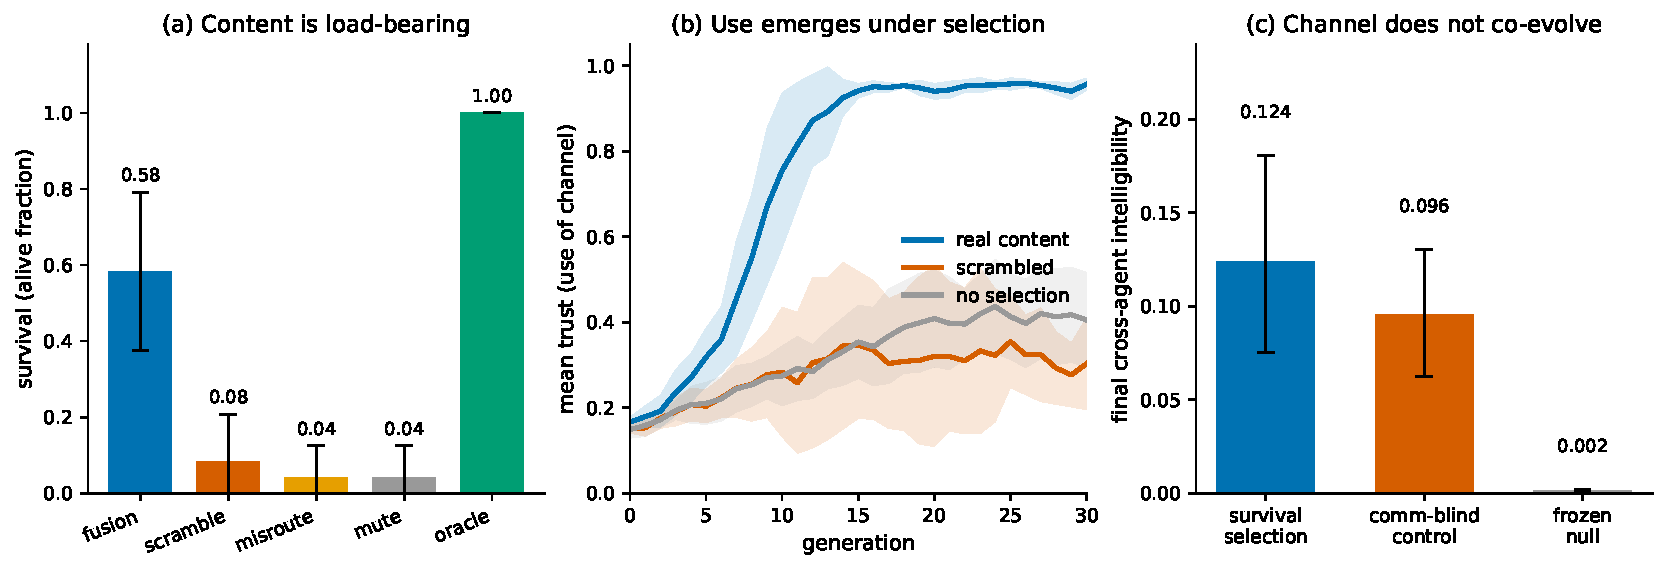
\includegraphics[width=\textwidth]{fig_rtc}
\caption{Results inside the constructed world; all values from committed verdict
artifacts, bars are bootstrap 95\% CIs. \textbf{(a)} Lethal signaling (24 seeds):
\emph{fusion} (real decoded content, 0.58) survives far above \emph{scramble}
(random, 0.08), \emph{misroute} (correct content, broken content-to-location
binding, 0.04) and \emph{mute} (0.04); \emph{oracle} (fenced) $=1.00$. fusion beats
each control by an exact paired McNemar test ($p<5\mathrm{e}{-}4$); the run's own
absolute-majority gate is inconclusive, so this is a \emph{relative} result, and
\emph{misroute} isolates that content-to-location \emph{binding} (not signal
presence) carries survival. \textbf{(b)} A heritable ``trust'' gene (8 seeds) rises
to ${\approx}0.96$ under real content vs.\ ${\sim}0.3$--$0.4$ under scrambled / no
selection: \emph{use} of a separately-trained channel is selected for (adoption,
not de-novo emergence). \textbf{(c)} Co-evolving the channel from random weights
(6 seeds): the apparent intelligibility rise (0.124) does \emph{not} separate from a
communication-blind control (0.096; survival$-$control CI $[-0.05, 0.11]$ includes
$0$), both far above the frozen null (0.002)---clonal descent-convergence, not
selection for communication.}
\label{fig:rtc}
\end{figure*}

\section{Constructively closing the shortcuts}
We build a world (a Relay-Tide Commons, RTC) that forecloses each shortcut by
construction, and test the residue with the same rig (\Cref{fig:rtc}).

\textbf{Natural foraging.} Grown-channel \emph{content} is \emph{not}
load-bearing: any movement-prompt suffices because foraging en route makes
message content irrelevant---a content-free shortcut at the survival layer.

\textbf{Lethal signaling (shortcuts foreclosed).} With no local sensing and a
forced lethal choice, grown-channel content---specifically its
content-to-location binding---becomes load-bearing \emph{relative} to degraded
controls (\Cref{fig:rtc}a); the decisive \emph{misroute} control (correct content,
broken binding) dies, so content, not signal presence, carries survival. Scope:
relative not absolute, inside a narrow stakes window, in a world built to make
content matter.

\textbf{Use emerges under selection.} A heritable trust gene gating message use
rises from $0.17$ to $0.96$ under real content, versus ${\sim}0.3$--$0.4$ under
scrambled content or no selection (\Cref{fig:rtc}b): selection for \emph{using} a
separately-trained channel (adoption), not de-novo emergence.

\textbf{Does the channel co-evolve?---a clean negative.} From random
speaker/listener weights under survival selection alone (no truth gradient), even
the strongest legitimate mechanism (tied encode/decode weights plus kin
assimilation) does not grow a load-bearing channel (\Cref{fig:rtc}c): the apparent
intelligibility rise did not separate from a communication-blind control, so it is
clonal descent-convergence, not selection for communication.

\section{Boundaries and contribution}
The positives live inside constructed worlds; the core goal---a load-bearing
grounded language that \emph{grows} from scratch under selection---is not
achieved. The recurring obstacle is world design plus a grounding/fidelity
ceiling: a grown channel can carry information yet remain too imprecise, or too
easily bypassed, to be load-bearing. We contribute (1)~a transferable adversarial
self-audit protocol that demonstrably catches false positives; (2)~a
precisely-mapped wall system; and (3)~a constructive recipe (close shortcuts, then
test) with scoped positives and a clean co-evolution negative. We suggest
emergent-communication claims be reported against architecture-matched nulls and
communication-blind controls as standard. All verdicts and code are committed;
headline scripts were independently rerun from a fresh clone on a separate machine
and produced the same verdicts, with an oracle-leakage audit. AI agents generated
implementation candidates and adversarial critiques, but all headline verdicts are
script-produced, committed, and reproducible from fixed seeds; the adversarial
multi-agent audit is itself part of the contribution.

\FloatBarrier
\footnotesize
\begin{thebibliography}{9}
\setlength{\itemsep}{0pt}
\bibitem[Chaabouni et al.(2020)]{chaabouni} Chaabouni, R., et al. (2020). Compositionality and generalization in emergent languages. \emph{ACL}.
\bibitem[Foerster et al.(2016)]{foerster} Foerster, J., et al. (2016). Learning to communicate with deep multi-agent reinforcement learning. \emph{NeurIPS}.
\bibitem[Geirhos et al.(2020)]{geirhos} Geirhos, R., et al. (2020). Shortcut learning in deep neural networks. \emph{Nature Machine Intelligence}.
\bibitem[Kirby et al.(2015)]{kirby} Kirby, S., Tamariz, M., Cornish, H., and Smith, K. (2015). Compression and communication in the cultural evolution of linguistic structure. \emph{Cognition}.
\bibitem[Lazaridou and Baroni(2020)]{lazaridou2020} Lazaridou, A., and Baroni, M. (2020). Emergent multi-agent communication in the deep learning era. \emph{arXiv:2006.02419}.
\bibitem[Lazaridou et al.(2017)]{lazaridou2017} Lazaridou, A., Peysakhovich, A., and Baroni, M. (2017). Multi-agent cooperation and the emergence of (natural) language. \emph{ICLR}.
\bibitem[Lehman and Stanley(2011)]{lehman} Lehman, J., and Stanley, K. O. (2011). Abandoning objectives: evolution through the search for novelty alone. \emph{Evolutionary Computation}.
\bibitem[Lewis(1969)]{lewis} Lewis, D. (1969). \emph{Convention}. Harvard University Press.
\bibitem[Locatello et al.(2019)]{locatello} Locatello, F., et al. (2019). Challenging common assumptions in the unsupervised learning of disentangled representations. \emph{ICML}.
\bibitem[Nowak(2006)]{nowak} Nowak, M. A. (2006). Five rules for the evolution of cooperation. \emph{Science}.
\bibitem[Ren et al.(2020)]{ren} Ren, Y., et al. (2020). Compositional languages emerge in a neural iterated learning model. \emph{ICLR}.
\bibitem[Skyrms(2010)]{skyrms} Skyrms, B. (2010). \emph{Signals: Evolution, Learning, and Information}. Oxford University Press.
\bibitem[Steels(2003)]{steels} Steels, L. (2003). Evolving grounded communication for robots. \emph{Trends in Cognitive Sciences}.
\end{thebibliography}

\end{document}
